%%%%%%%%%%%%%%%%%%%%%%%%%%%%%%%%%%%%%%%%%%%%%%%%%%%%%%%%%%%%%%%%%%%%%%%%%%%%%%%%
%2345678901234567890123456789012345678901234567890123456789012345678901234567890
%        1         2         3         4         5         6         7         8

\documentclass[letterpaper, 10 pt, conference]{ieeeconf}  % Comment this line out if you need a4paper

%\documentclass[a4paper, 10pt, conference]{ieeeconf}      % Use this line for a4


\IEEEoverridecommandlockouts                              % This command is only needed if 
                                                          % you want to use the \thanks command

\overrideIEEEmargins                                      % Needed to meet printer requirements.

% See the \addtolength command later in the file to balance the column lengths
% on the last page of the document

% The following packages can be found on http:\\www.ctan.org
%\usepackage{graphics} % for pdf, bitmapped graphics files
%\usepackage{epsfig} % for postscript graphics files
%\usepackage{mathptmx} % assumes new font selection scheme installed
%\usepackage{times} % assumes new font selection scheme installed
%\usepackage{amsmath} % assumes amsmath package installed
%\usepackage{amssymb}  % assumes amsmath package installed
\usepackage[utf8]{inputenc}
\usepackage[english]{babel}
\usepackage{graphicx}
\title{\LARGE \bf
 Clinic Subject Management Hybrid Application
}


\author{\IEEEauthorblockN{{Kim bosung}}
\IEEauthorblockA{\\Information System Dept. \\College of Engineering\\
Hanyang Univ\\
Seoul, Korea REP.\\
bosung2697@gmail.com}\and
\IEEEauthorblockN{Nam yunwoo}
\IEEauthorblockA{\\Information System Dept. \\College of Engineering\\
Hanyang Univ\\
Seoul, Korea REP.\\
kikis93@naver.com}\and
\IEEEauthorblockN{Jeong Sujin}
\IEEauthorblockA{\\Information System Dept. \\College of Engineering\\
Hanyang Univ\\
Seoul, Korea REP.\\
wjdtnwls1011@gmail.com}\and
\IEEEauthorblockN{Ha Dongsu}
\IEEauthorblockA{\\Information System Dept. \\College of Engineering\\
Hanyang Univ\\
Seoul, Korea REP.\\
gkehdtn4218@hanmail.net}\and
\IEEEauthorblockN{Kim Eunhye}
\IEEauthorblockA{\\Information System Dept. \\College of Engineering\\
Hanyang Univ\\
Seoul, Korea REP.\\
gracekim510@naver.com}
}





\begin{document}


\maketitle
\thispagestyle{empty}
\pagestyle{empty}


%%%%%%%%%%%%%%%%%%%%%%%%%%%%%%%%%%%%%%%%%%%%%%%%%%%%%%%%%%%%%%%%%%%%%%%%%%%%%%%%
\begin{abstract}

Using Clinical Subject Management(CSM), Hanyang laboratories can easily find people they need and keep their data. For Students, they can find proper part-time job.

\end{abstract}


%%%%%%%%%%%%%%%%%%%%%%%%%%%%%%%%%%%%%%%%%%%%%%%%%%%%%%%%%%%%%%%%%%%%%%%%%%%%%%%%

\section{INTRODUCTION}
\maketitle{\textit{Motivation\\}}

Because there was no platform that could communicate between Hanyang lab and students, it is hard for researcher to find clinical subjects. They find subjects through personal ways. For example, receiving text or mail one by one in their own phone. So we want to create a platform that allows the lab to post recruitment notice and students to look at it and apply for what they want. And Because there were no such things that manage their experimental data, we add one more thing in our app. A simple database system. Researchers can keep their test result or subjects’ personal data efficiently. 

\maketitle{\textit{\\Related Software}}

\subsection{Albamon}

It Is one of the most famous applications for students to search part-time job. It provides information of various jobs. Job seekers can set up your own interests and receive push notifications for that. And they can fill out their resumes to keep it in the app.

\subsection{Olive C}
This application makes it easy to provide recent clinical information. People can participate in that clinical test if it’s good for themselves. There are Different things between Olive C and our application. CSM  is only used in Hanyang Lab, and it can database the result of the clinic




\section{REQUIREMENT ANALYSIS\\}


\subsection{Account Management}
\subsubsection{Separate Account Data}
There are two types of users. The lab researchers and applicants for experiments. For each of the user, different front page will be shown that contains different functions. At the very first page, users have to choose whether they are lab researchers or applicants. 
\subsubsection{Sign Up}
For the lab researcher member, it is required to register the lab and his or her e-mail address. When it is first time to make account of the lab itself, the page for the lab will be created. Otherwise, the user has to select the preregistered lab and send request to the general manager of the lab. Then the request e-mail will be sent to the manager. After approving, the user's account is created. For the applicants, they have to enter their e-mail address, name and phone number. This information will be delivered to researchers who manage the experiment that the applicant applies. 
\subsubsection{Log In}
After clicking whether they are lab researchers or applicants at the very first page, log in page will be shown. Users can sign in with their e-mail address and password. Buttons for password will be provided.


\subsection{Functions For Lab}

\subsubsection{Main Page}
The experiment schedule of the lab will be shown in the form of calender.  Also, the list of experiment instances will be shown with check box. There is another list that shows all the researcher registered in that lab. The general manger has authority with this list. There are four buttons one for creating new experiment instance, another for searching the previous data of specific experiment, another for posting recruitment notice and the other for uploading/revising experiment result data. 
After checking one of the check box at the list of experiment instances, it is possible to click one of the last three buttons. 
\subsubsection{Experiment Data Query}
If a researcher selects one of the experiments in the list and click the searching button at the main page, the page of querying for that experiment data will be shown. The user can easily search for specific experiment data according to the name of subjects, date, the researcher in charge and the objective of the experiment. 
\subsubsection{Uploading/Revising Experiment Result Data}
If a researcher selects one of the experiments in the list and click this button at the main page, the page of uploading and revising for the experiment result data will be shown. The researcher in charge can enter the date,time, explanatory comment, name and other special features of the subject. It is also possible to request for personal information like age and gender. 
\subsubsection{Create Experiment Instance}
After clicking the button for creation of new experiment instance at the main page, pop-up for entering specific information of the new experiment will be shown. Only the general manager can use this function. The name of the researcher in charge, experiment objective and the name and type of the experiment should be entered. 
\subsubsection{Posting the Recruitment Notice}
After clicking the button for posting recruitment notice at the main page, the researcher in charge moves to the next page. In this page, the researcher should make the schedule of the experiment date and time via calender UI. Then the researcher should enter the specific information like the payment, condition, the method of experiment, place of the laboratory, expected duration time. The notice form delivered to the applicants page will automatically include these details in addition to name of the experiment, name of the researcher in charge, date and time. This notice form will be loaded to the applicants' main page.

\subsection{Functions For Applicants}
\subsubsection{Main Page}
In this page, users can see the list of recruitment notices in a similar form like Albamon. They can search specific experiment by setting conditions like the type,payment and date. The list can be organized in order of payment and deadline.
\subsubsection{Detail Information Page}
If users click one of the recruitment notices, they move to the next page which contains details of the experiment. It shows the information that are entered by the researcher in charge. Additionally, there is a calender combined with check box. The applicant should first check one of the check boxes and click apply button. This apply button will show pop-up with the message of "successfully applied" and the list of previously applied experiments. There is another button for inquiry message.



\subsection{Communication Between Applicants and Lab}
\subsubsection{Message Drop Box}
If applicant wants to reschedule or make inquiries, sending direct message will be useful. With this service, the researchers do not need to reply with their own phone or e-mail. 
\subsubsection{Communication page for Lab}
This page shows the list of scheduled experiments. The elements can be divided according to whether there are applicants or not. There is pop-up notice that tell them every time someone apply for the experiment. Also, there is drop box which contain all the inquiry messages from applicant and reply to them. 
\subsubsection{Communication page for Applicants}
After clicking the inquiry message button at the page of detailed information, pop-up will be shown to enter inquiry message. This message will be saved in the account's drop box. 


\section{\\DEVELOPMENT ENVIRONMENT}
\subsection{Choice of software development platform}

\maketitle{\textit{Form of application: Hybrid Application}}

We were trying to create an application only. However, we figured out that the application alone is not sufficient for users and the laboratory side to write and post a notice. To be specific, the main problem is that the data file which the lab researchers handle is not a simple text. In most cases, the file format is .bdf and .mat. These data files are usually stored at the desktop computer in the lab. If we create mobile application, it will be difficult to deliver the file from desktop to the server. Additionally, there are a lot of things to type in when posting a notice, entering personal information and so on. Therefore, we decided to make a hybrid application. We will make a web for the laboratory and use reaction type web for the mobile application. 

\maketitle{\textit{Programming Language}}

In order to develop the hybrid application, we decided to use Cordova Adobe Phonegap. PhoneGap is the original and most popular distribution of Apache Cordova. It will allow us to turn HTML, CSS and JavaScript into an app on our own device in minutes using the simple desktop and developer apps.With this tool, there is no need to handle android.
Additionally, we will use html and css to make web page’s basic and style, and decorate the web page using javascript (javascript 1.8.5), bootstrap and jQuery (jQuery 3.3.1). For the web framework, we will use Python Flask and PHP. In the back-end, we will use the JAVA (JAVA version 8 u191) language and MySQL to implement the database. 

\maketitle{\textit{Tool}}

In addition, we decided to use Kakao oven. This is used as a prototyping tool in the phase of making layout and designing UI in the front page. Each team member is going to communicate through this tool. The team member who took the responsibility of designer will mainly use this tool. 
For version control system, we are going to use bitbucket. Its service is free to the team which its number of members are less than 5. 


\begin{table}[h]
\caption{Cost Estimation}
\label{table_example}
\begin{center}
\begin{tabular}{|c||c|}
\hline
Device & Price( per month)\\
\hline
Amazon EC2 & 22\\
\hline
\end{tabular}
\end{center}
\end{table}

\maketitle{\textit{Platform}}

Each team member will use their own laptop with windows 10 home. 

\subsection{Software in use}
\subsubsection{olive c}
This is a smart clinical trial support service to help volunteers who want to participate in a clinical trial. Using this application, you can easily find clinical trials and check if you are adequate for the recent clinical trial.
\subsubsection{Github}
Github is a web-based hosting service for version control using Git. It is used for computer code. It offers all of the distributed version control and source code management functionality of Git as well as adding its own features. It provides access control and several collaboration features such as bug tracking, feature requests, task management, and wikis for every project.\\



\section{SPECIFICATIONS}

\subsection{Account Management}


MySQL database is required. Several schema will be needed;The list of lab researchers, applicants, registered lab, general manager of each lab, information of accounts like email-adress and password. At the very first page, users should whether they are lab researcher or applicant. After choosing their type, then the sign up and sign in page will be shown.
\graphicspath{{./Oven/}}

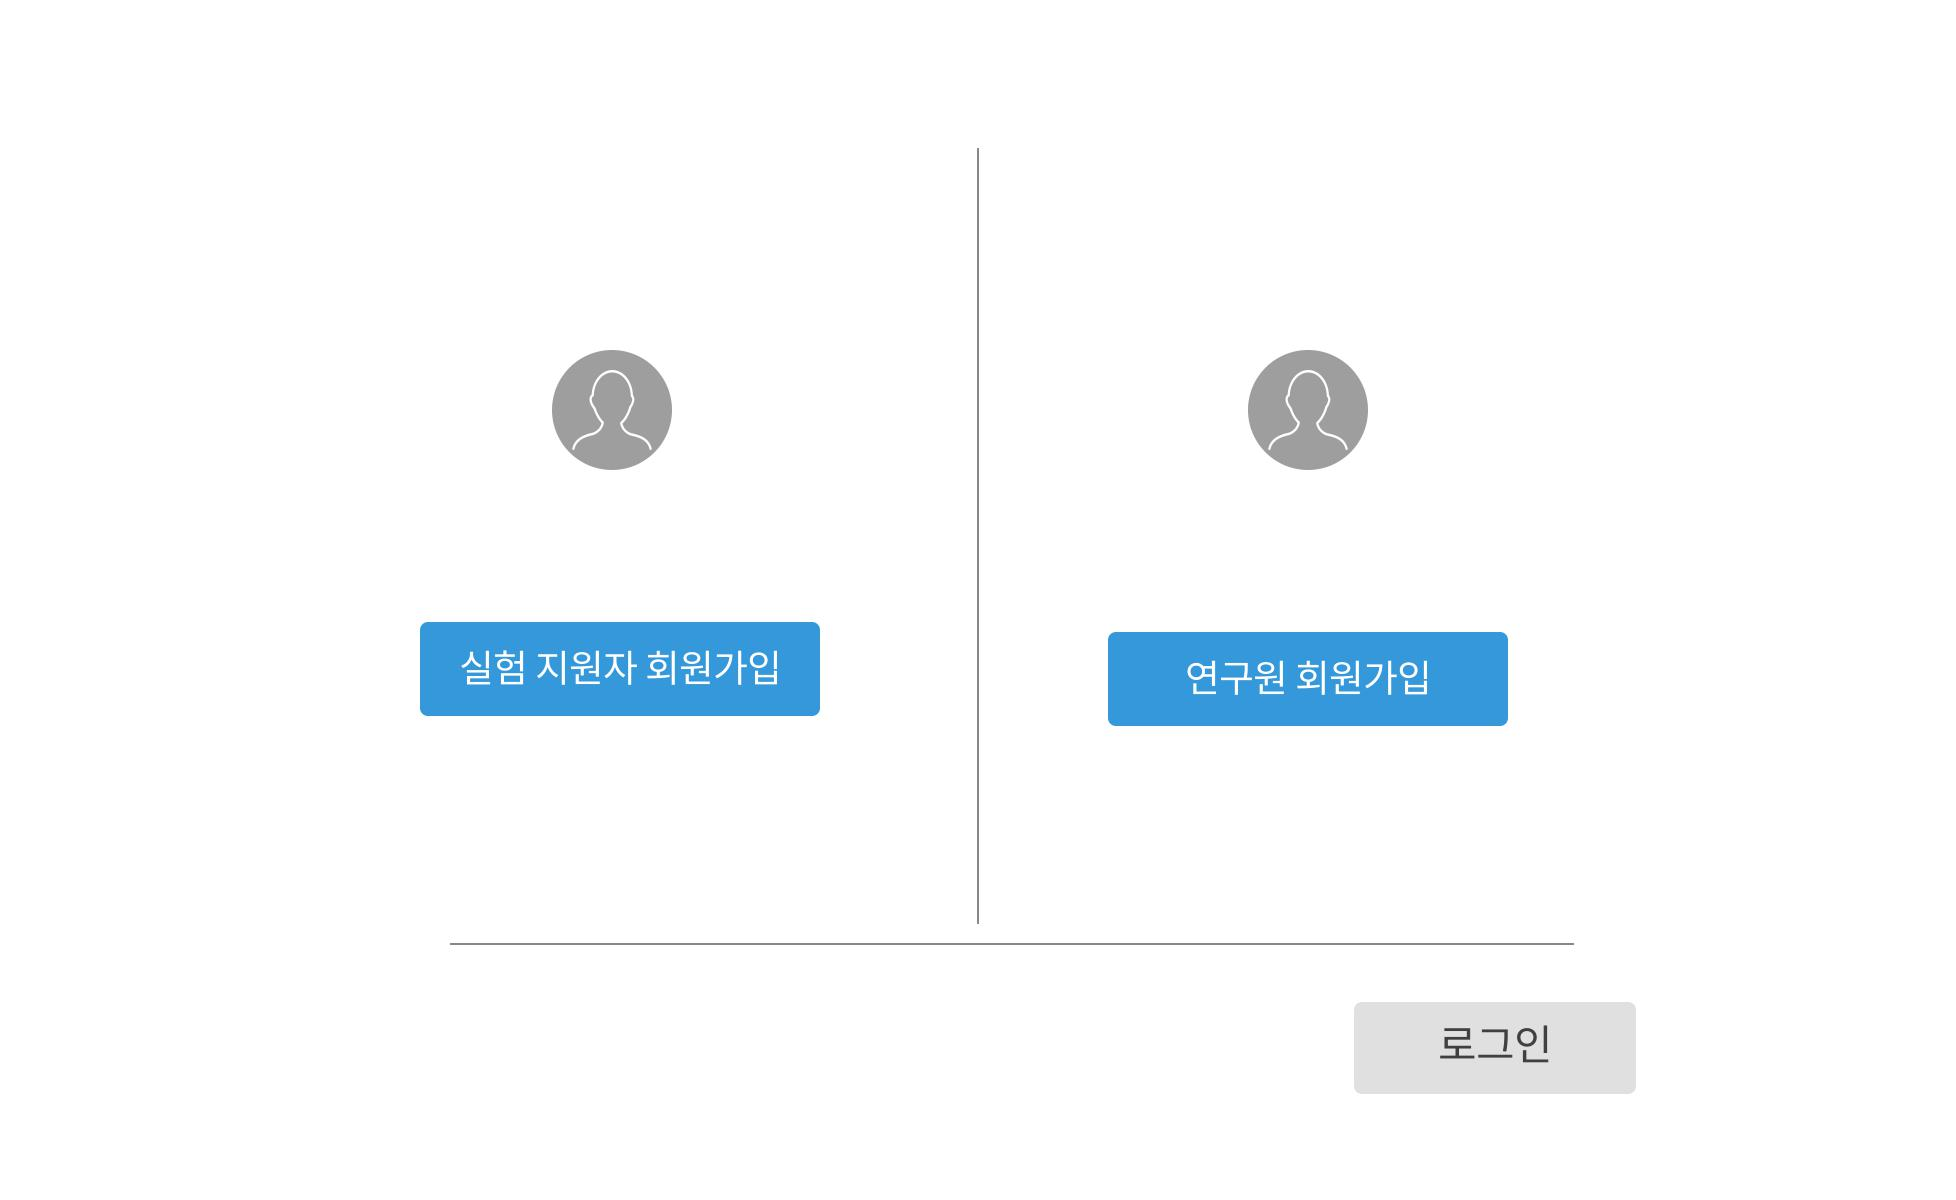
\includegraphics[width=8cm]{01_firstpage}


\subsubsection{Separate Account Data}
The information of users should be organized at MySQL database. Whether they registered as a lab researcher or applicants must be include in the column. The column which contains the type of the users will determine which of the two main pages will be selected at the server. 
\subsubsection{Sign Up}
Users can register with email address and password. For the lab researchers, it is needed to check first whether the lab is registered at the database table by the general manager. If it is the first time to register the lab, the first researcher type user that signs up will be authorized as general manager by default. If other researchers want to make account, they can search for the their lab in the database and check it. The request email will be sent to general manager's email address which are stored at database. 
If users click the button below, the homepage that says the sign up process is successfully done will be shown. In that page, users can click the log in button which will pop the sign-in pop up window.
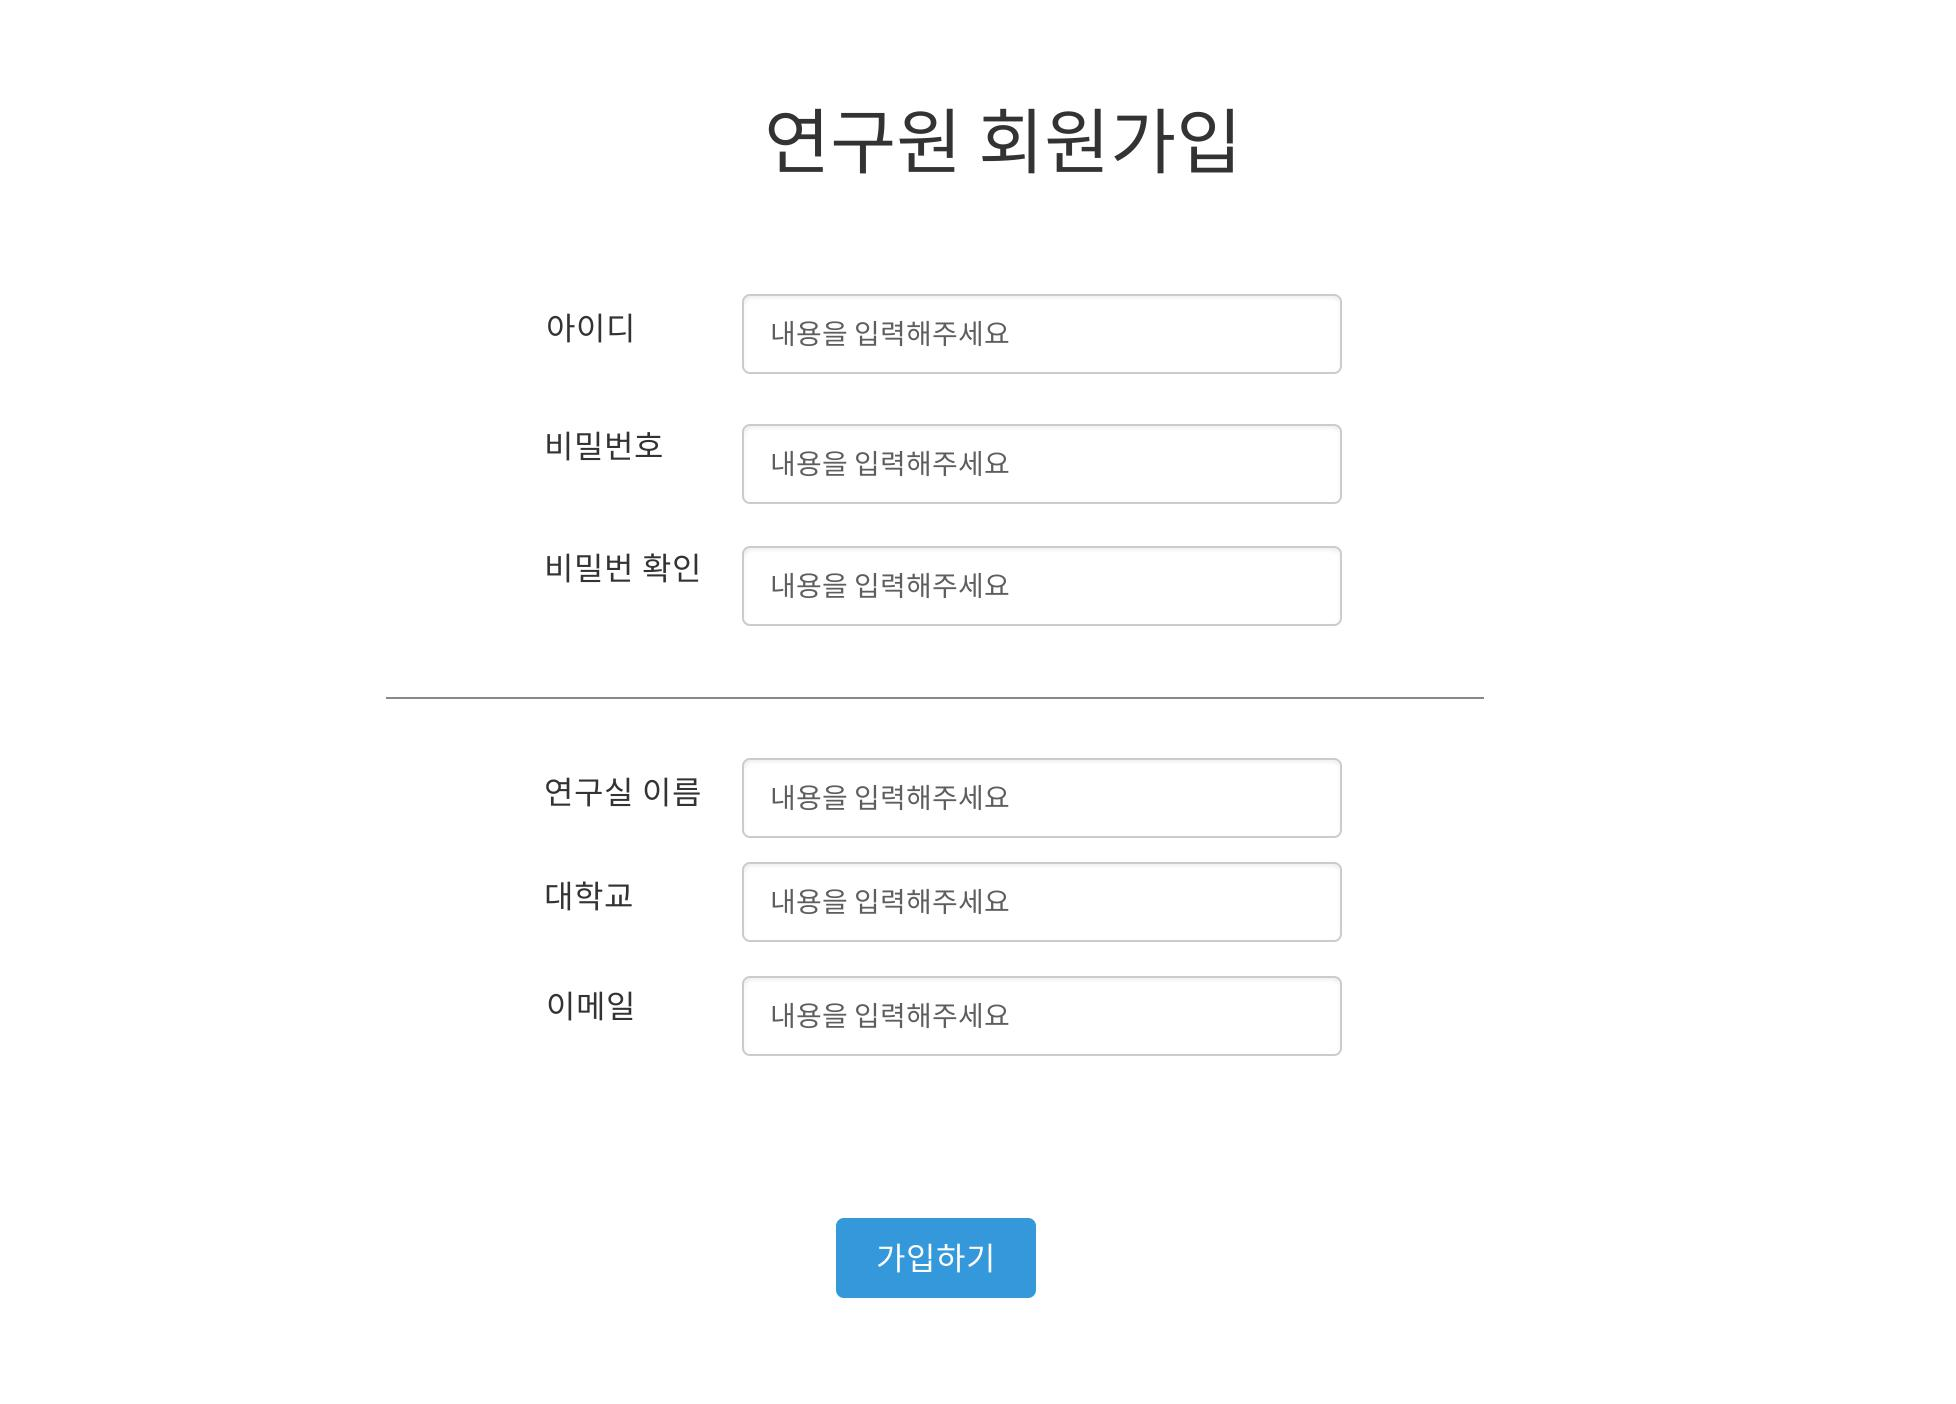
\includegraphics[width=6cm]{Oven/04_labSignup.jpg}
\subsubsection{Log in}
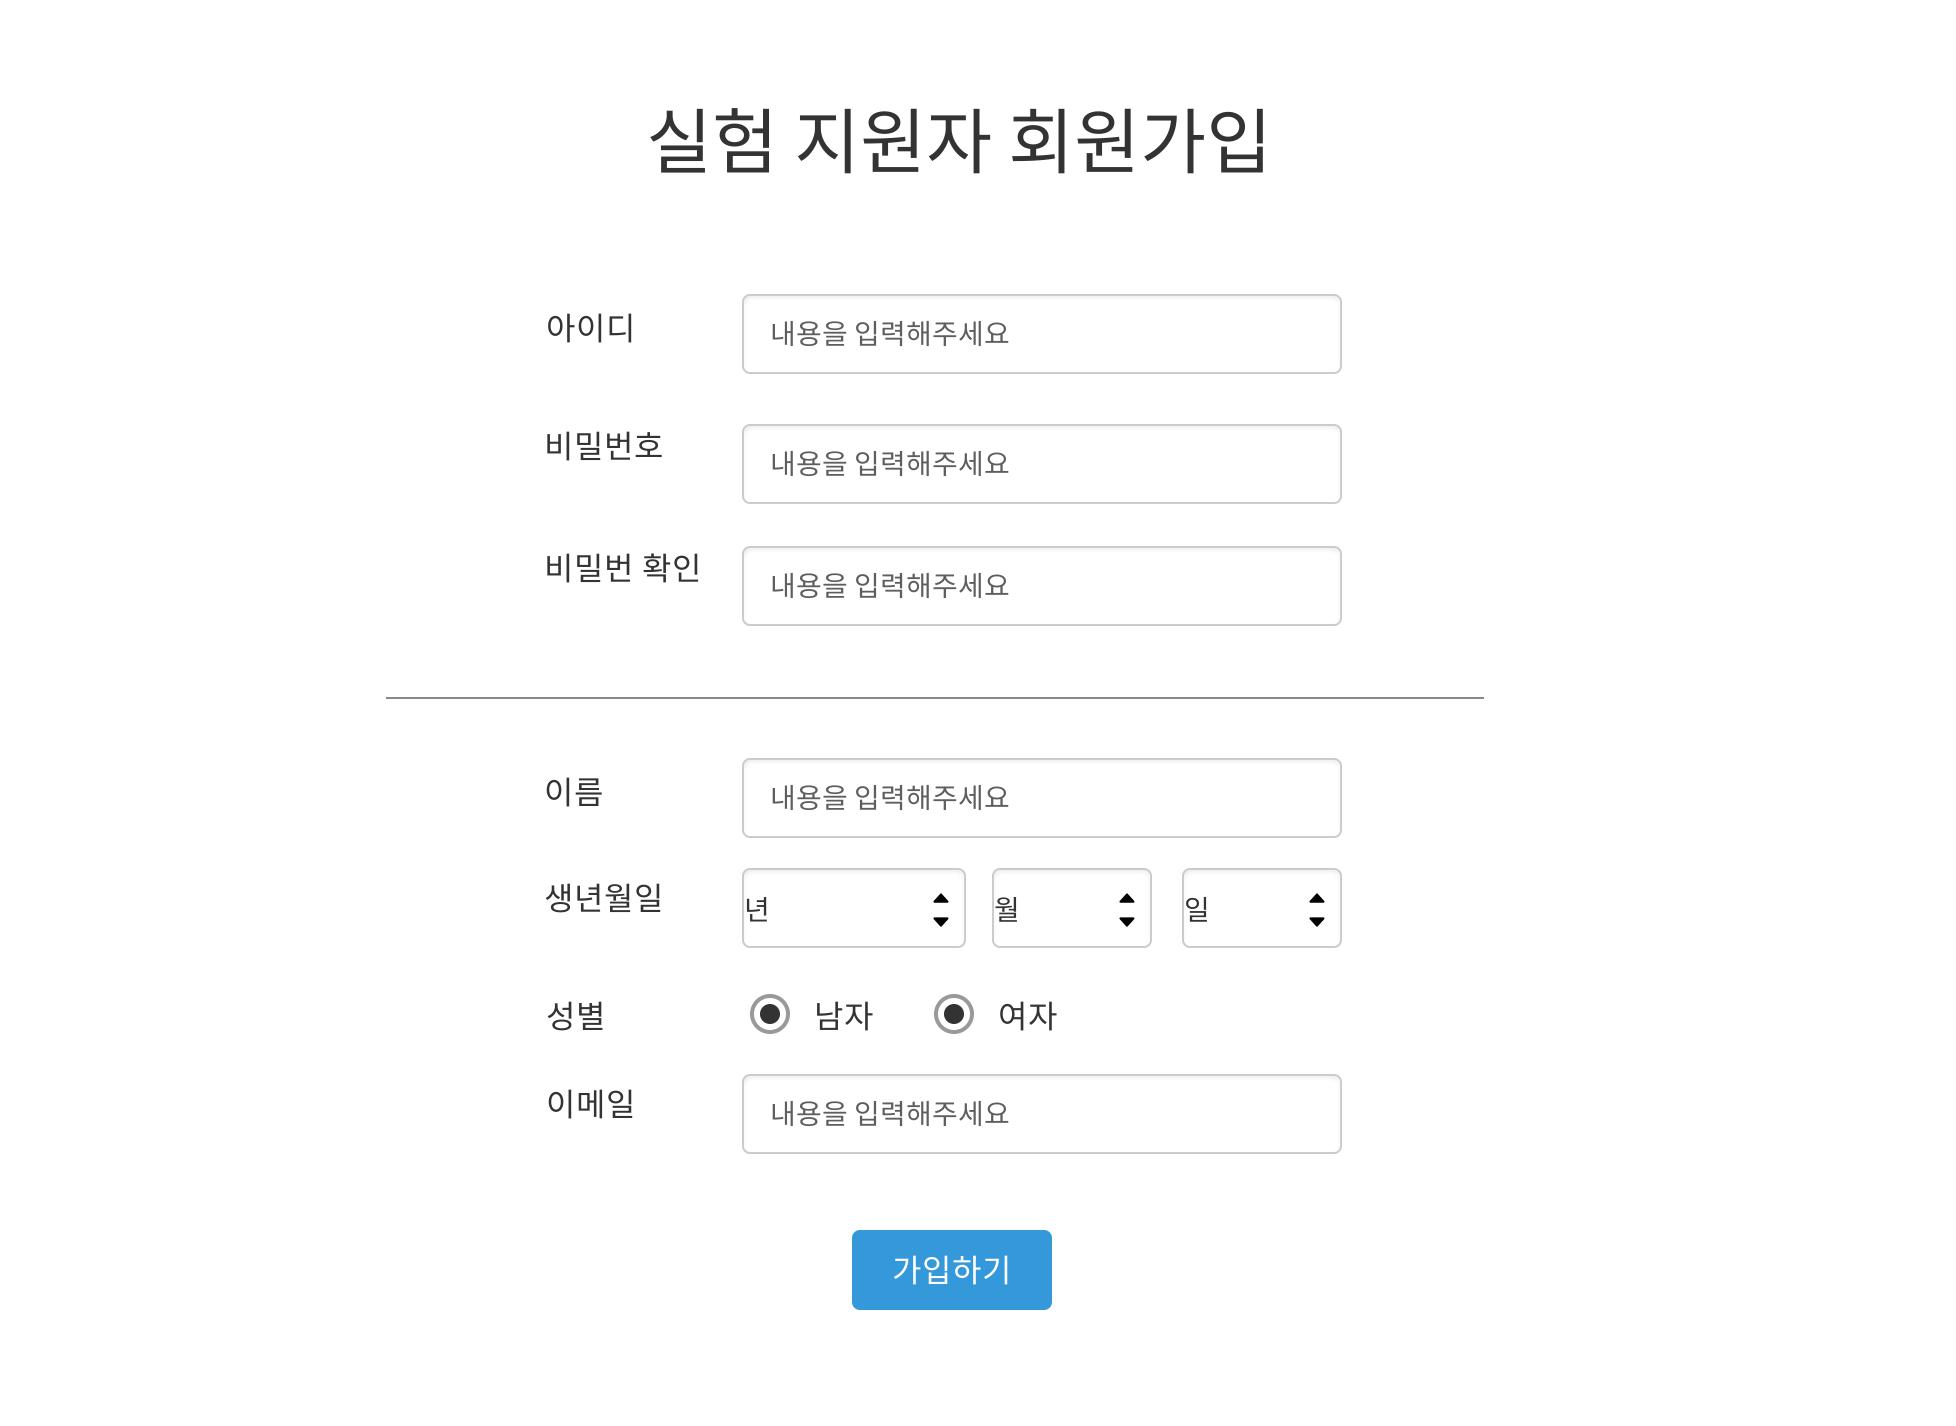
\includegraphics[width=6cm]{Oven/03_applicantSignup.jpg}
There is two radio buttons. Each of one indicates applicants and lab researcher. User has to one of these and enter ID and PW correctly. Then click the log in button. According to user's member type, main page for lab researcher or applicants will be shown.

\includegraphics[width=6cm]{Oven/05_signupCompleted.jpg}

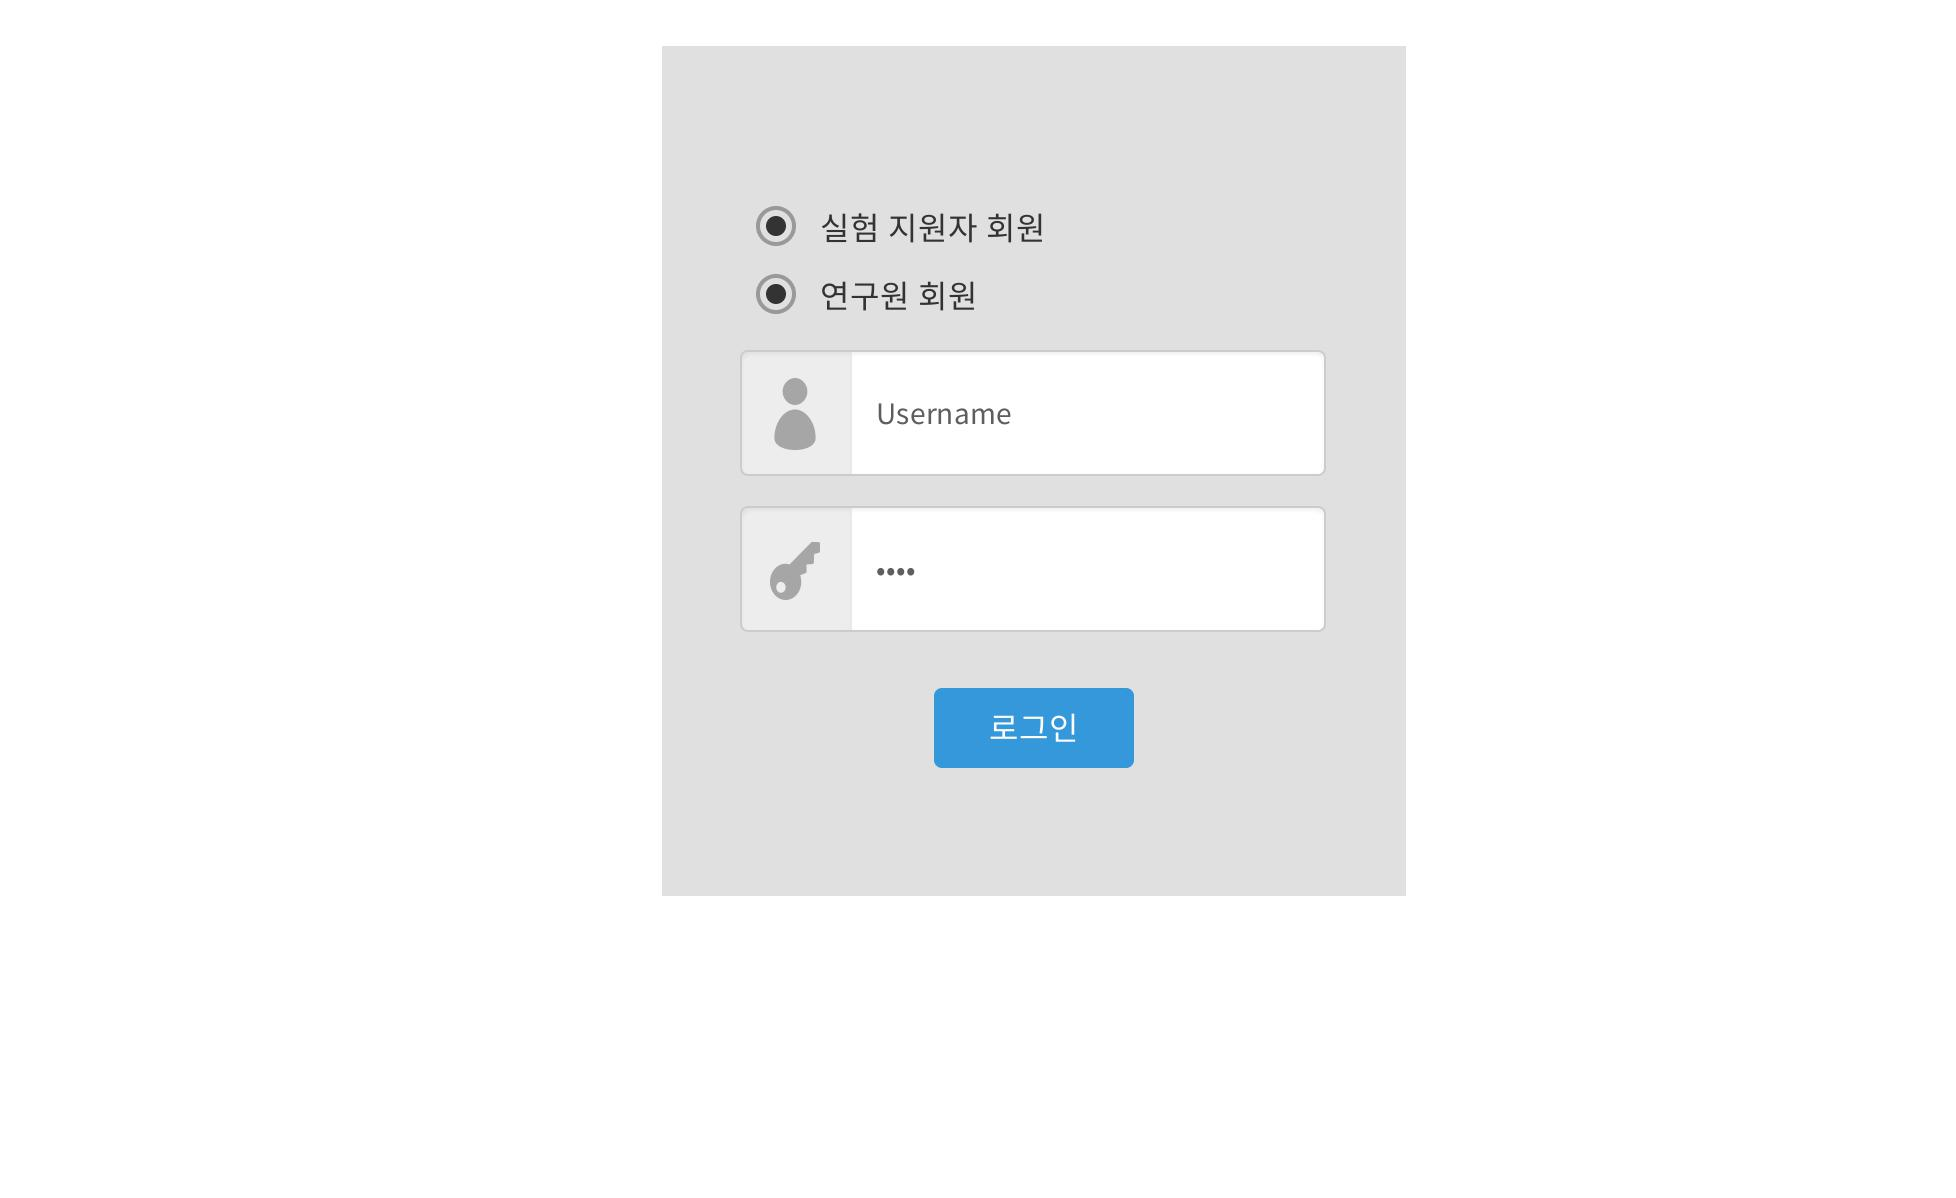
\includegraphics[width=6cm]{02_signin}



\subsection{Functions For Lab}

\subsubsection{Main Page\\}

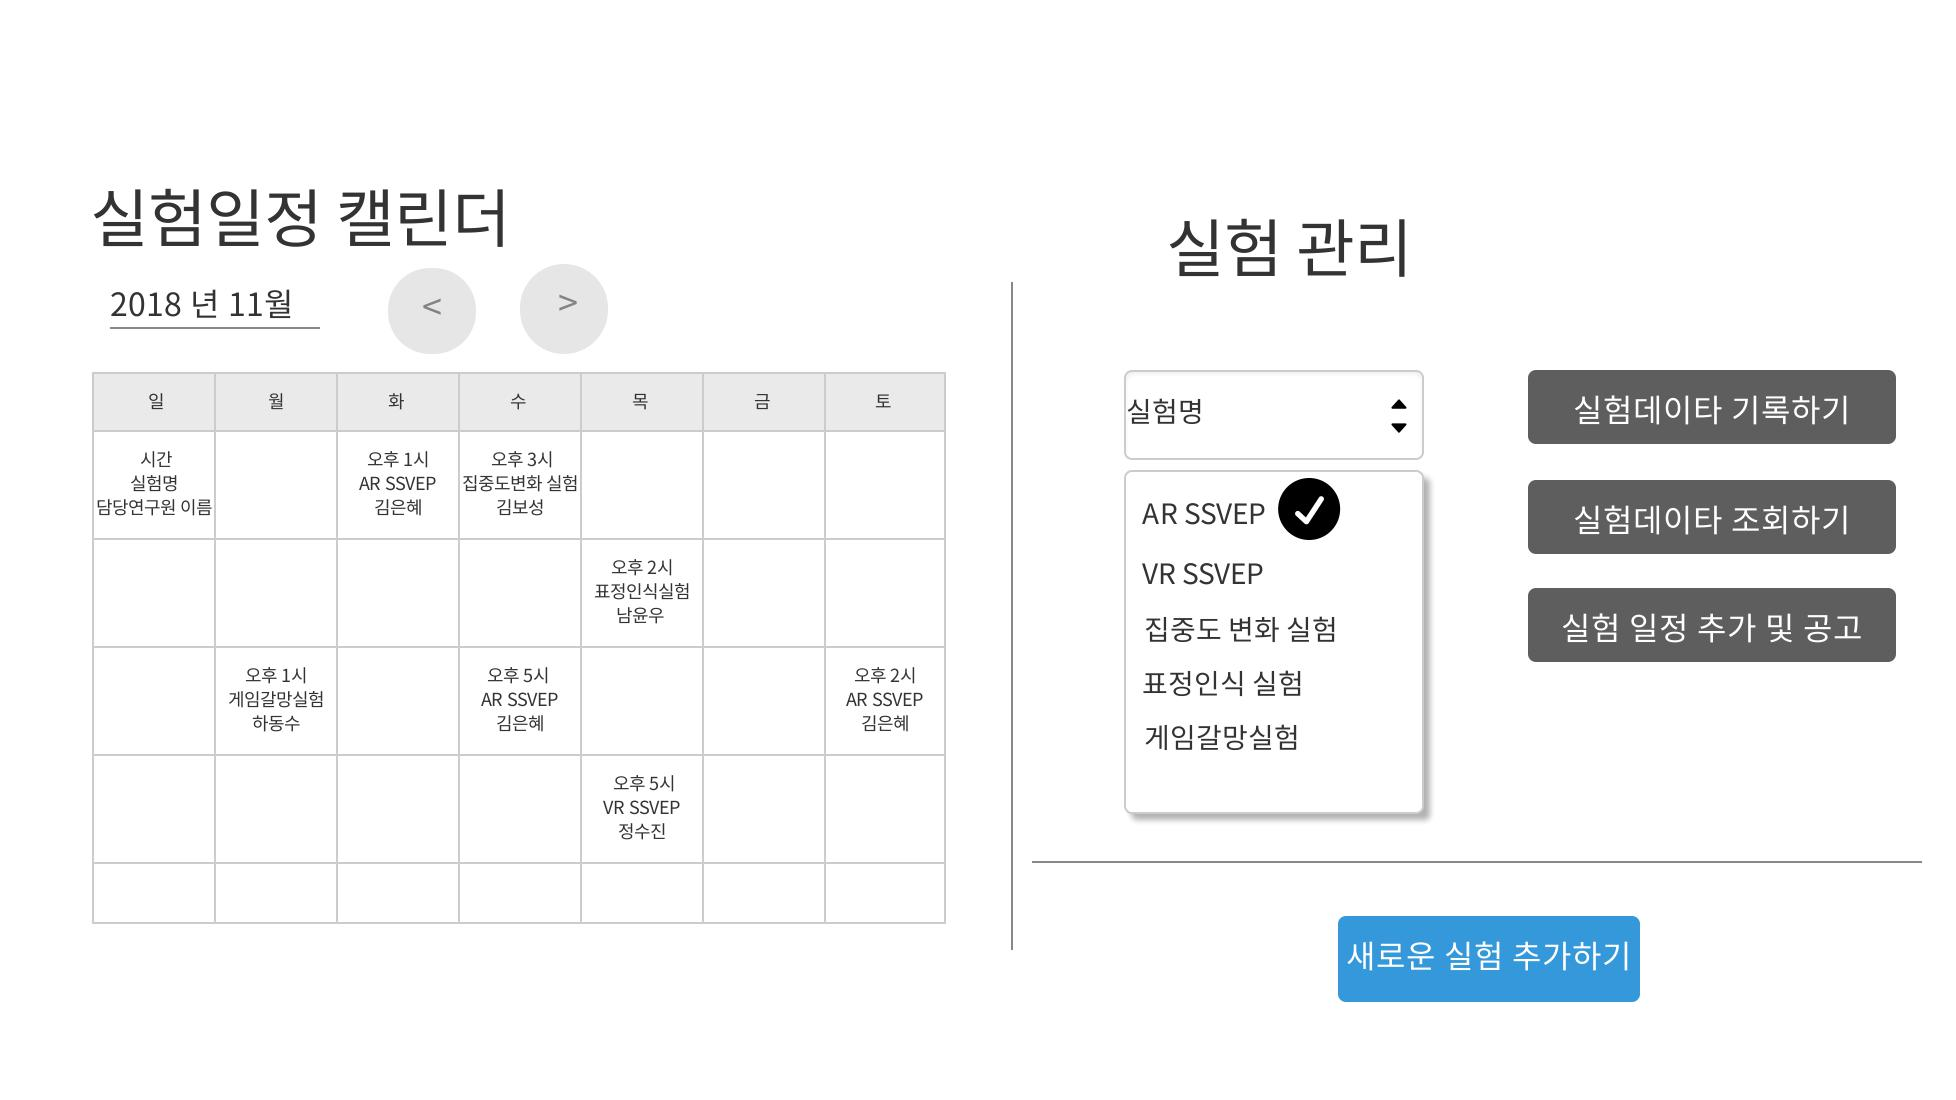
\includegraphics[width=6cm]{Oven/06-labMainpage.jpg}
\begin{itemize}
\item Experiment Schedule Calender : Similar as google calender. User can see all the scheduled experiments at the month at a glance. It also includes the experiment schedule that no applicants had applied. 
\item List of Experiment Instances With Drop Down List of Researchers In The Lab : This list will function as interface between main page and other functional pages. Just check one of the drop down elements and click the buttons below. 
\item Button For Creating New Experiment Instance
\item Button For Searching Previous Experiment Result Data
\item Button For Posting Recruitment Notice
\item Button For Uploading And Revising Experiment Result Data

\end{itemize}
\subsubsection{Experiment Data Query}
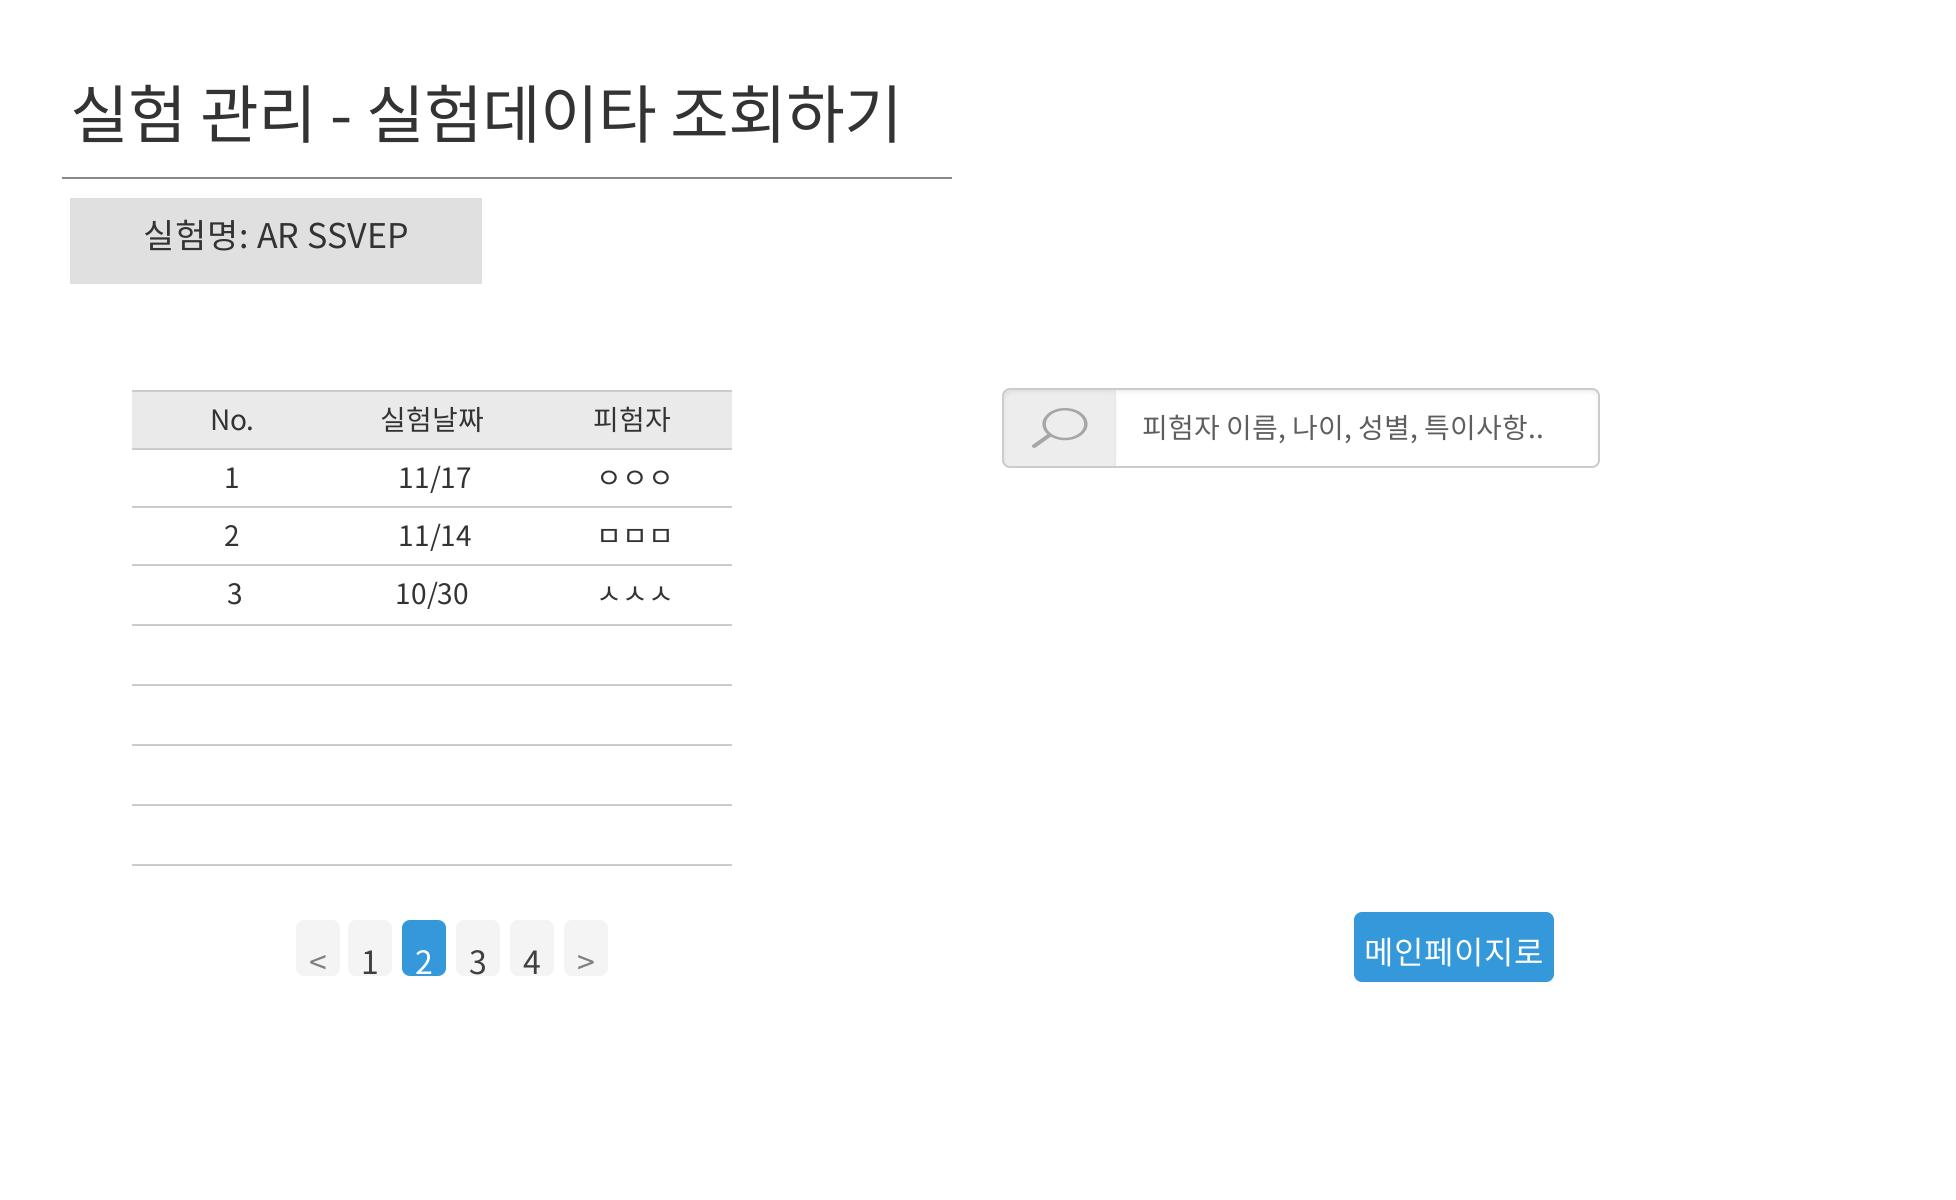
\includegraphics[width=6cm]{Oven/09_reviewingData.jpg}
 \\A table will be shown which contains all the date when the experiment is held. Recently held experiments will be at the top of table. Lab researchers can search for a specific data by entering several information of applicants or key words about that experiment. If they click one of the elements, pop up window will be shown which contains all the information about that experiment. 

\subsubsection{Uploading/Revising Experiment Result Data}
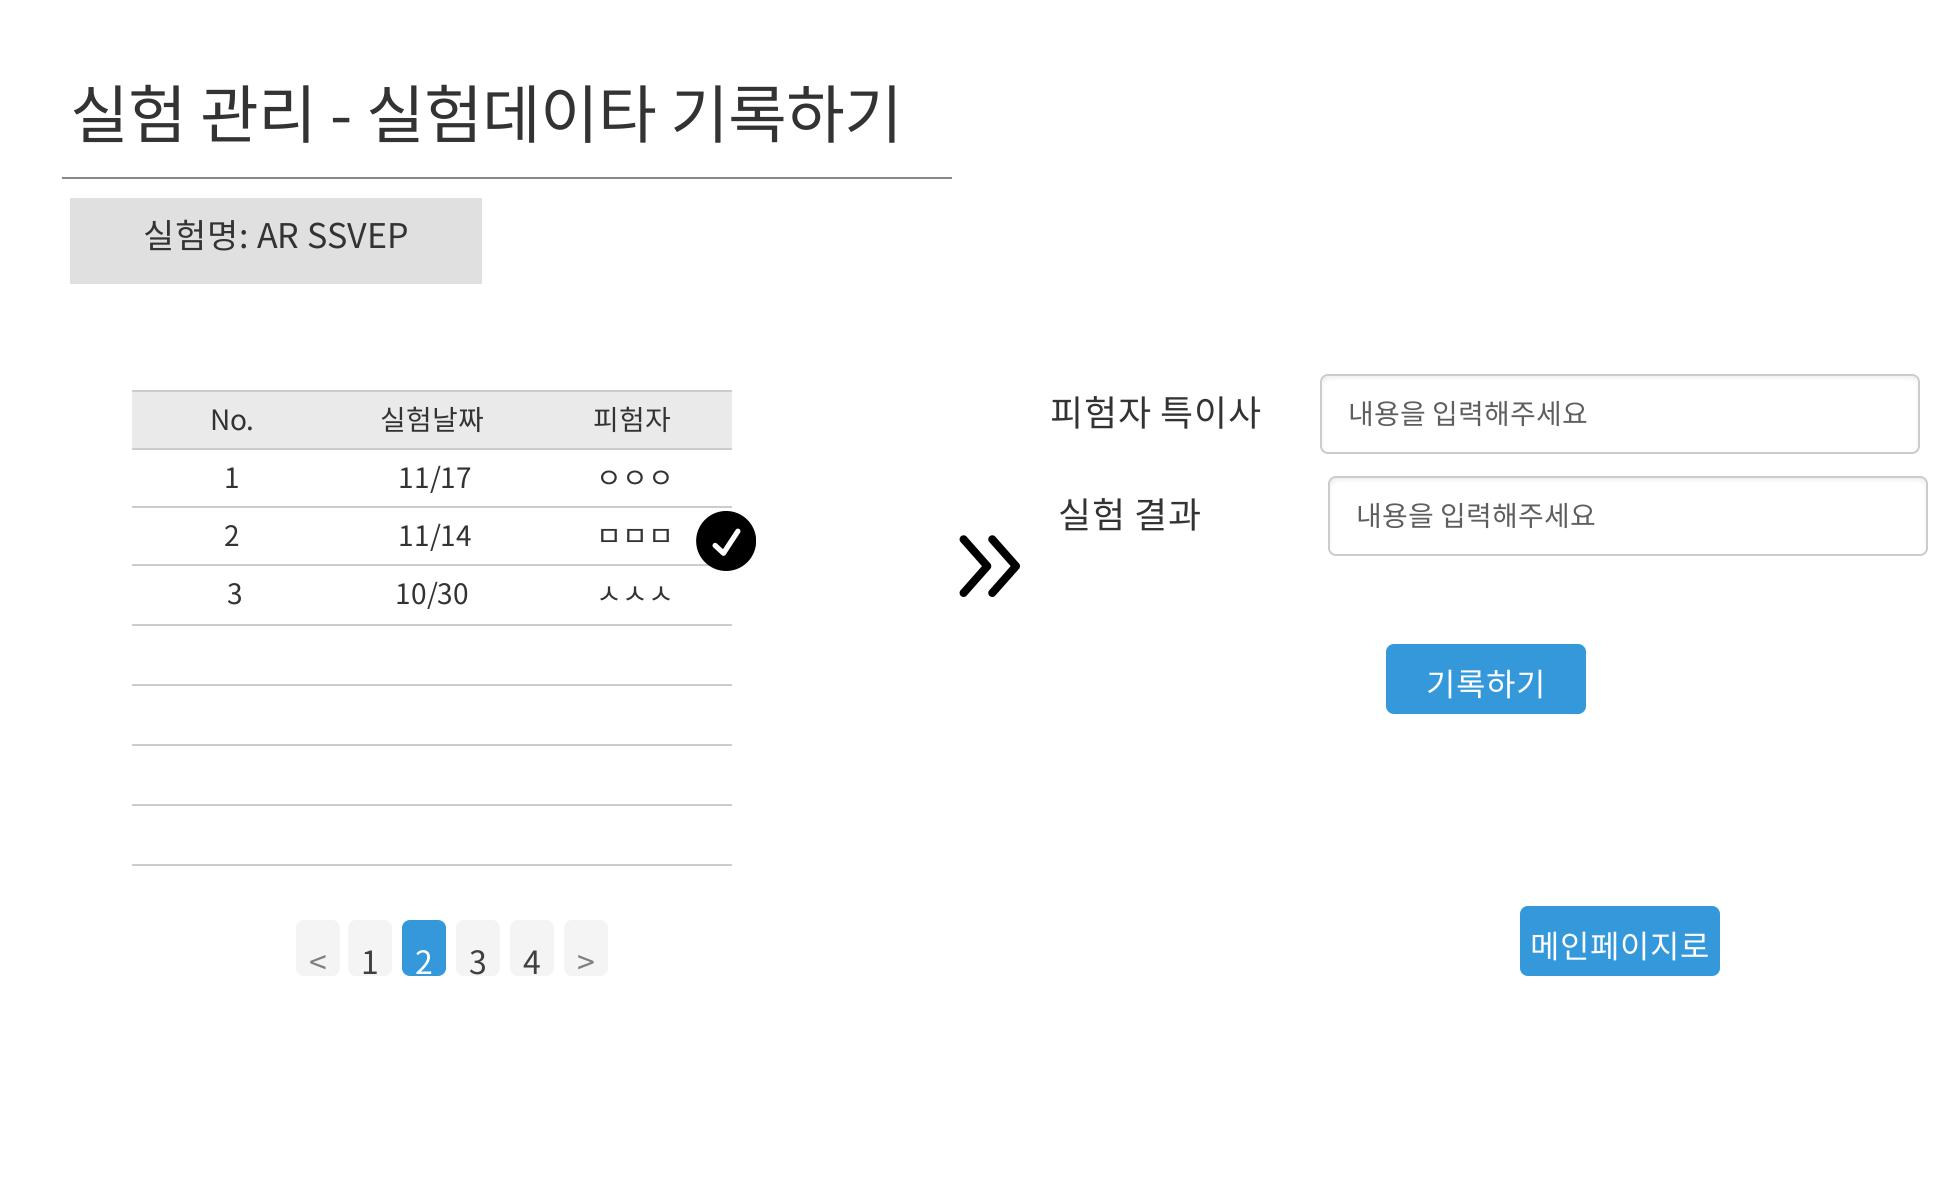
\includegraphics[width=6cm]{Oven/08_recordingData.jpg}
\\Same table of Experiment Data Query page will be shown. After clicking one of the elements, users can enter the specific features of applicants and result of experiment. 

\subsubsection{Create Experiment Instance}
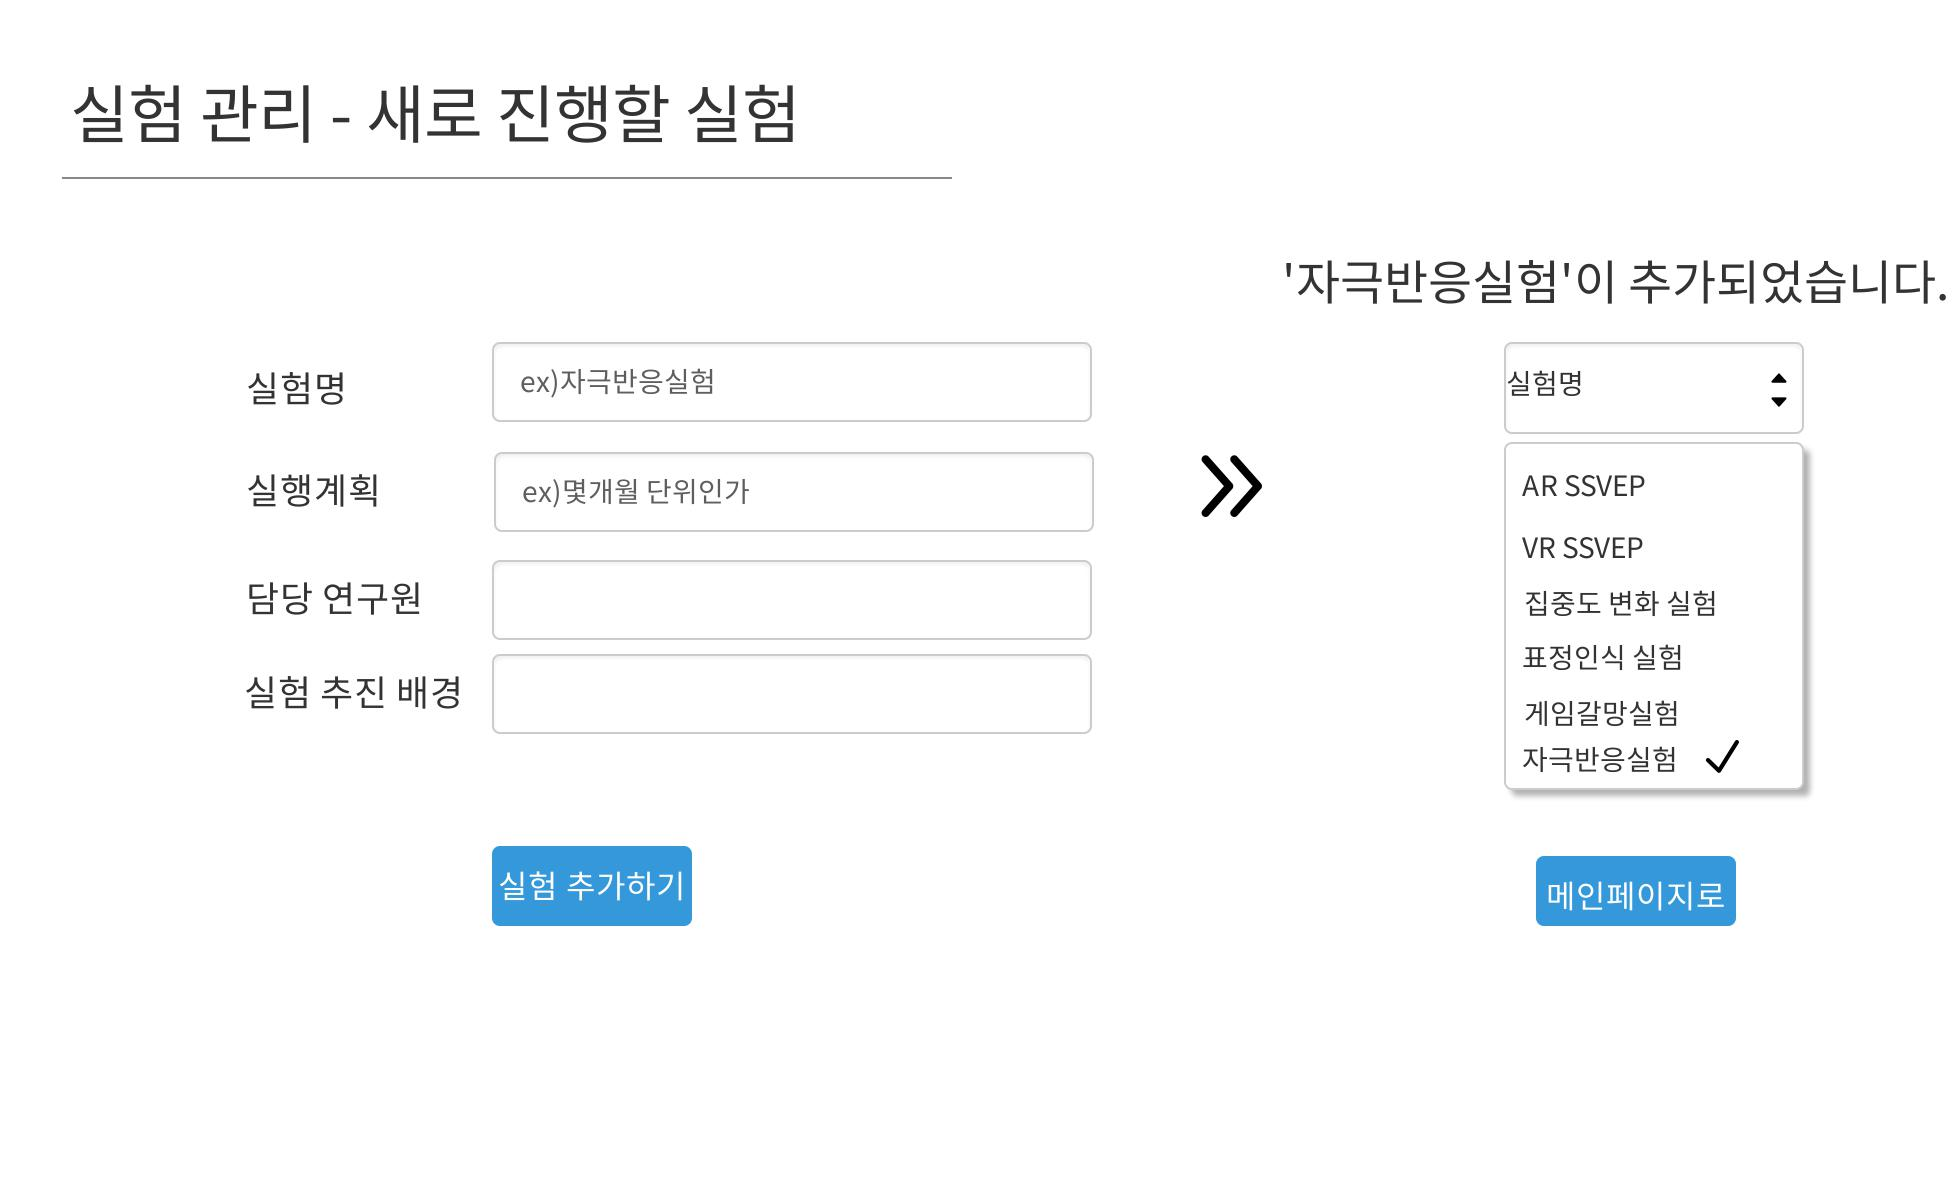
\includegraphics[width=6cm]{Oven/07_addNewExperiment.jpg}
\\When the lab researchers decided to hold a new type of experiment, the instance of that experiment should be created in database. Enter the name of experiment, expected schedule, researcher in charge and the purpose of it. 
\subsubsection{Posting the Recruitment Notice}
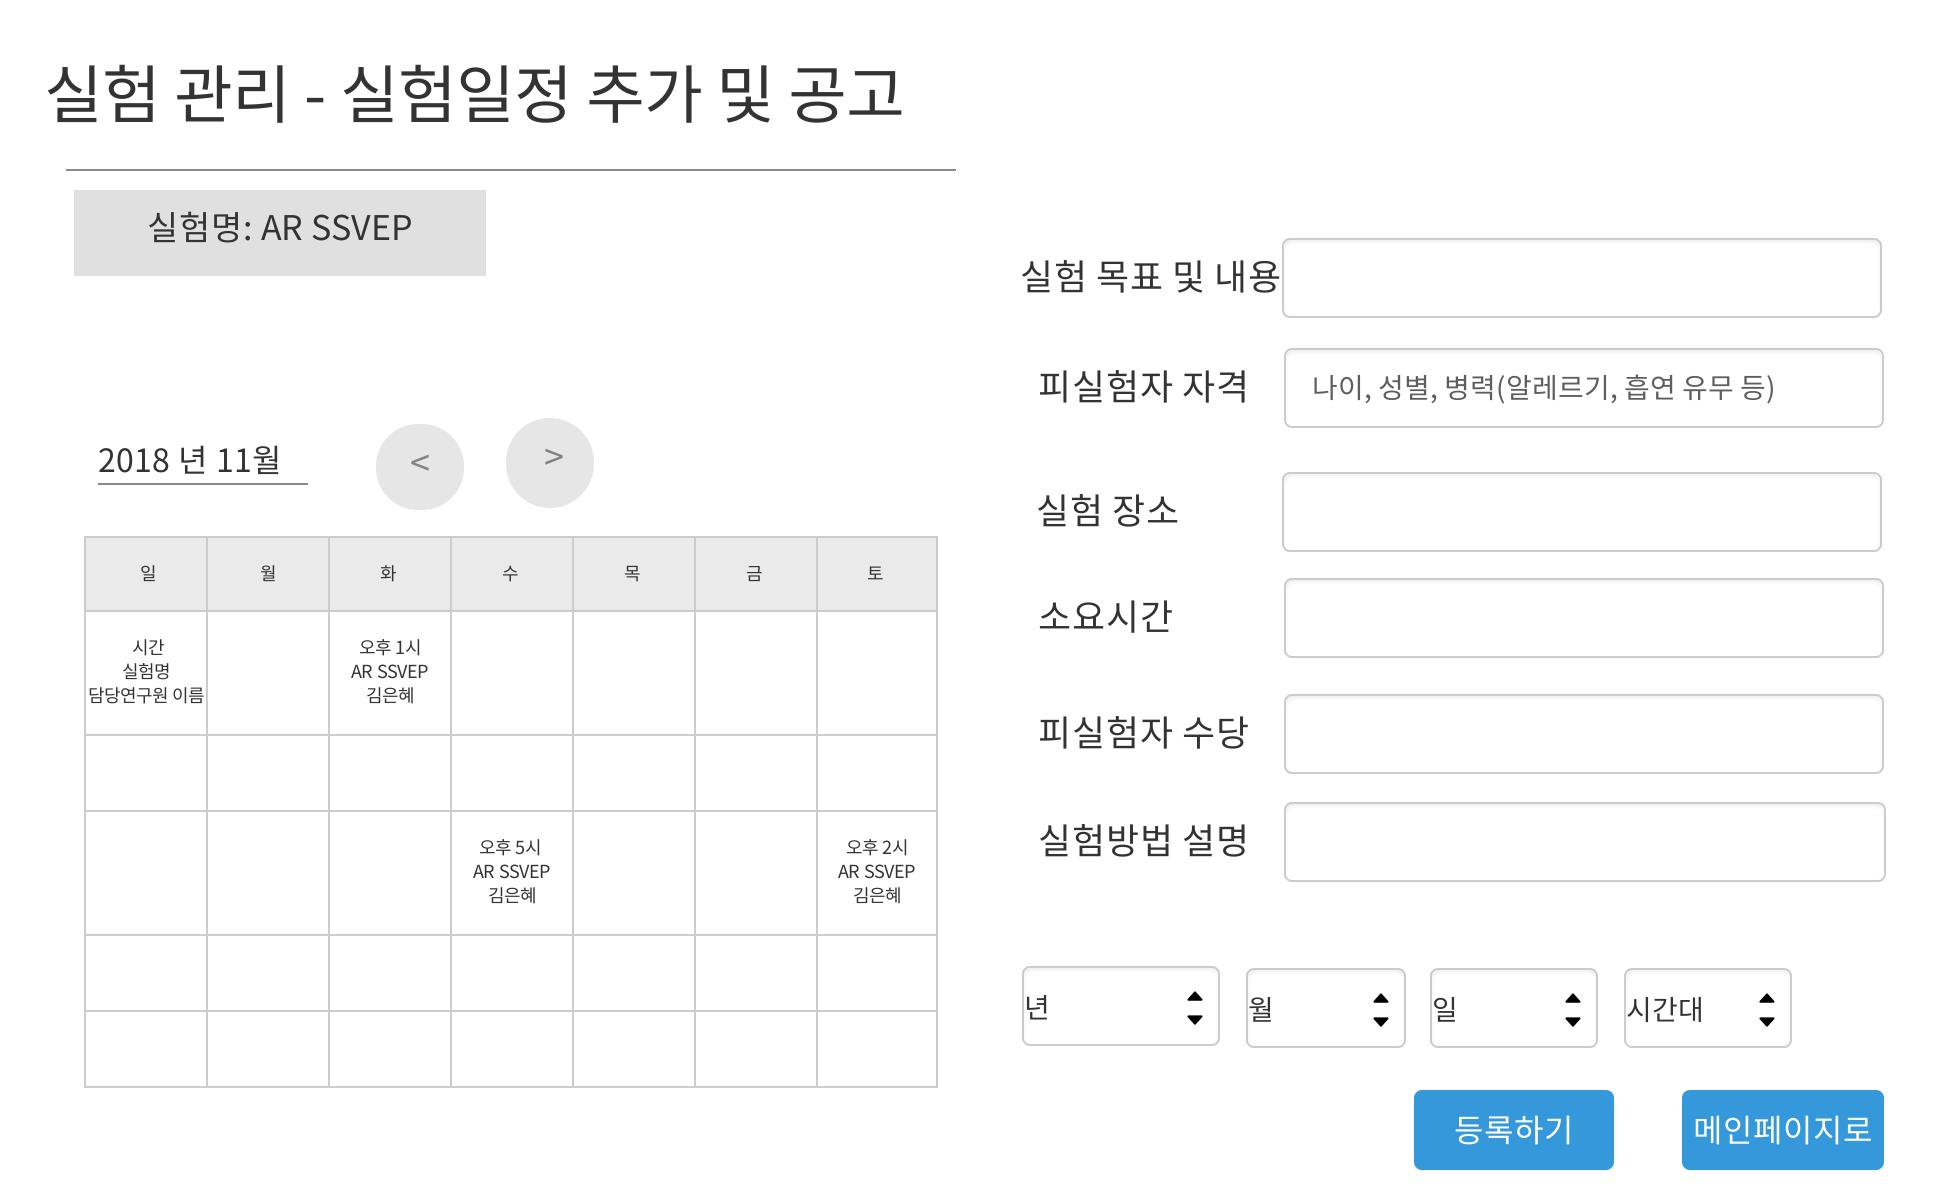
\includegraphics[width=6cm]{Oven/10_ScheduleNotice.jpg}
\\The scheduled experiments will be shown in the form of calender. Lab researchers can choose the day and time excluding previously scheduled day and time. They should type in the purpose of experiment, requirements for applicants, location, expected duration time, pay and the steps of experiment. All these information will instantly posted in the applicants' main page list in a well organized form as the button is clicked. 

\subsection{Functions For Applicants}
\subsubsection{Main Page\\}
\\Users can search for a specific experiment they prefer with key words like the name of experiment, related major or the name of university that the lab belongs to. At the top f list, recommended recruitment will be shown. Below this, the list of all the notices is located. This list is updated real time. If applicant click one of these elements, the page of Detailed Information Page will be shown. 

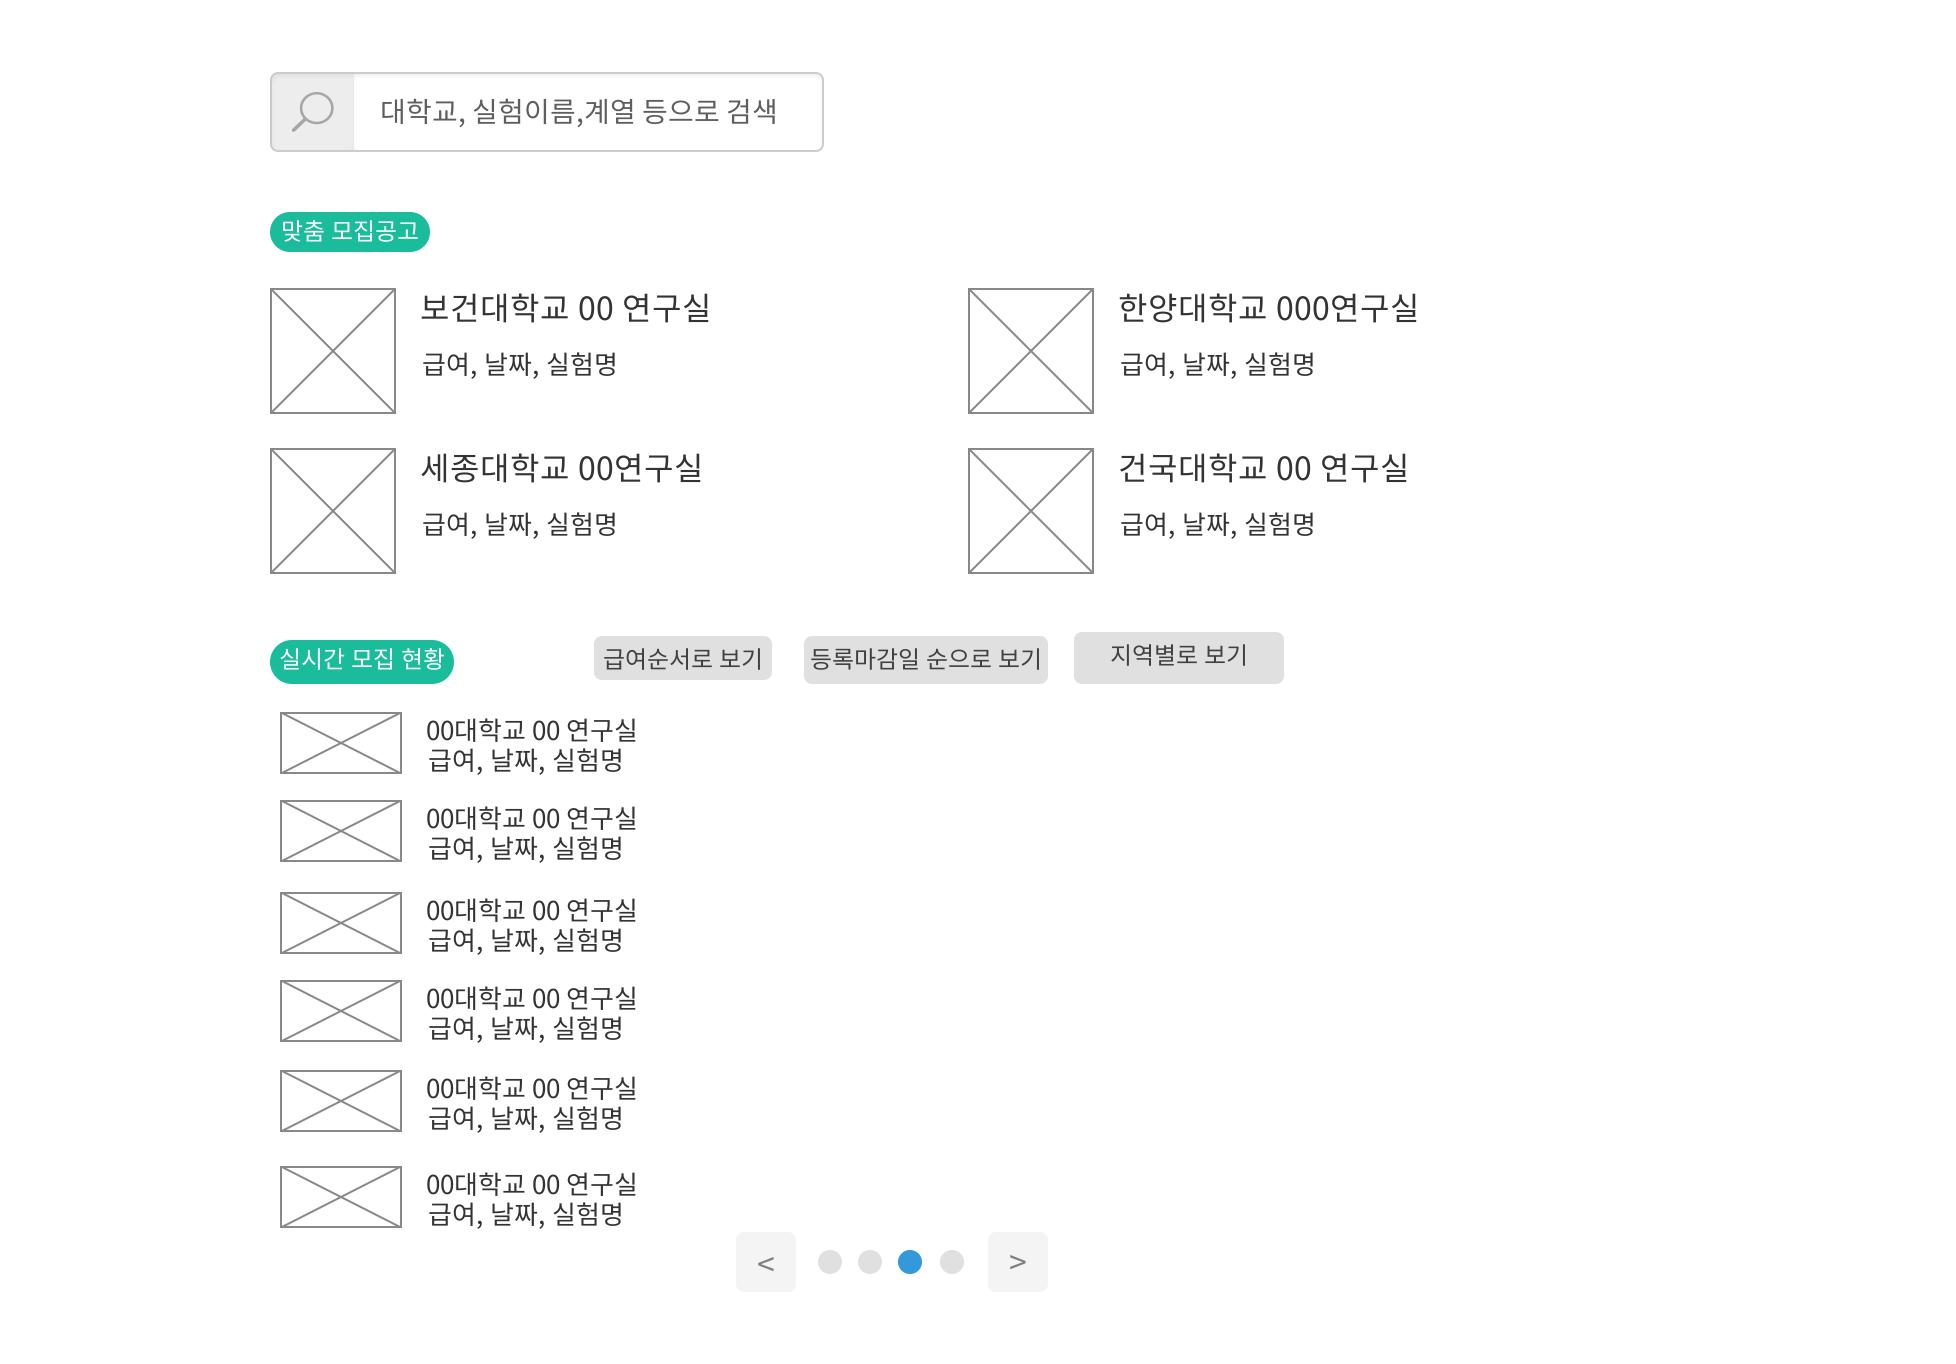
\includegraphics[width=6cm]{Oven/11_applicantMainpage.jpg}

\subsubsection{Detailed Information Page}
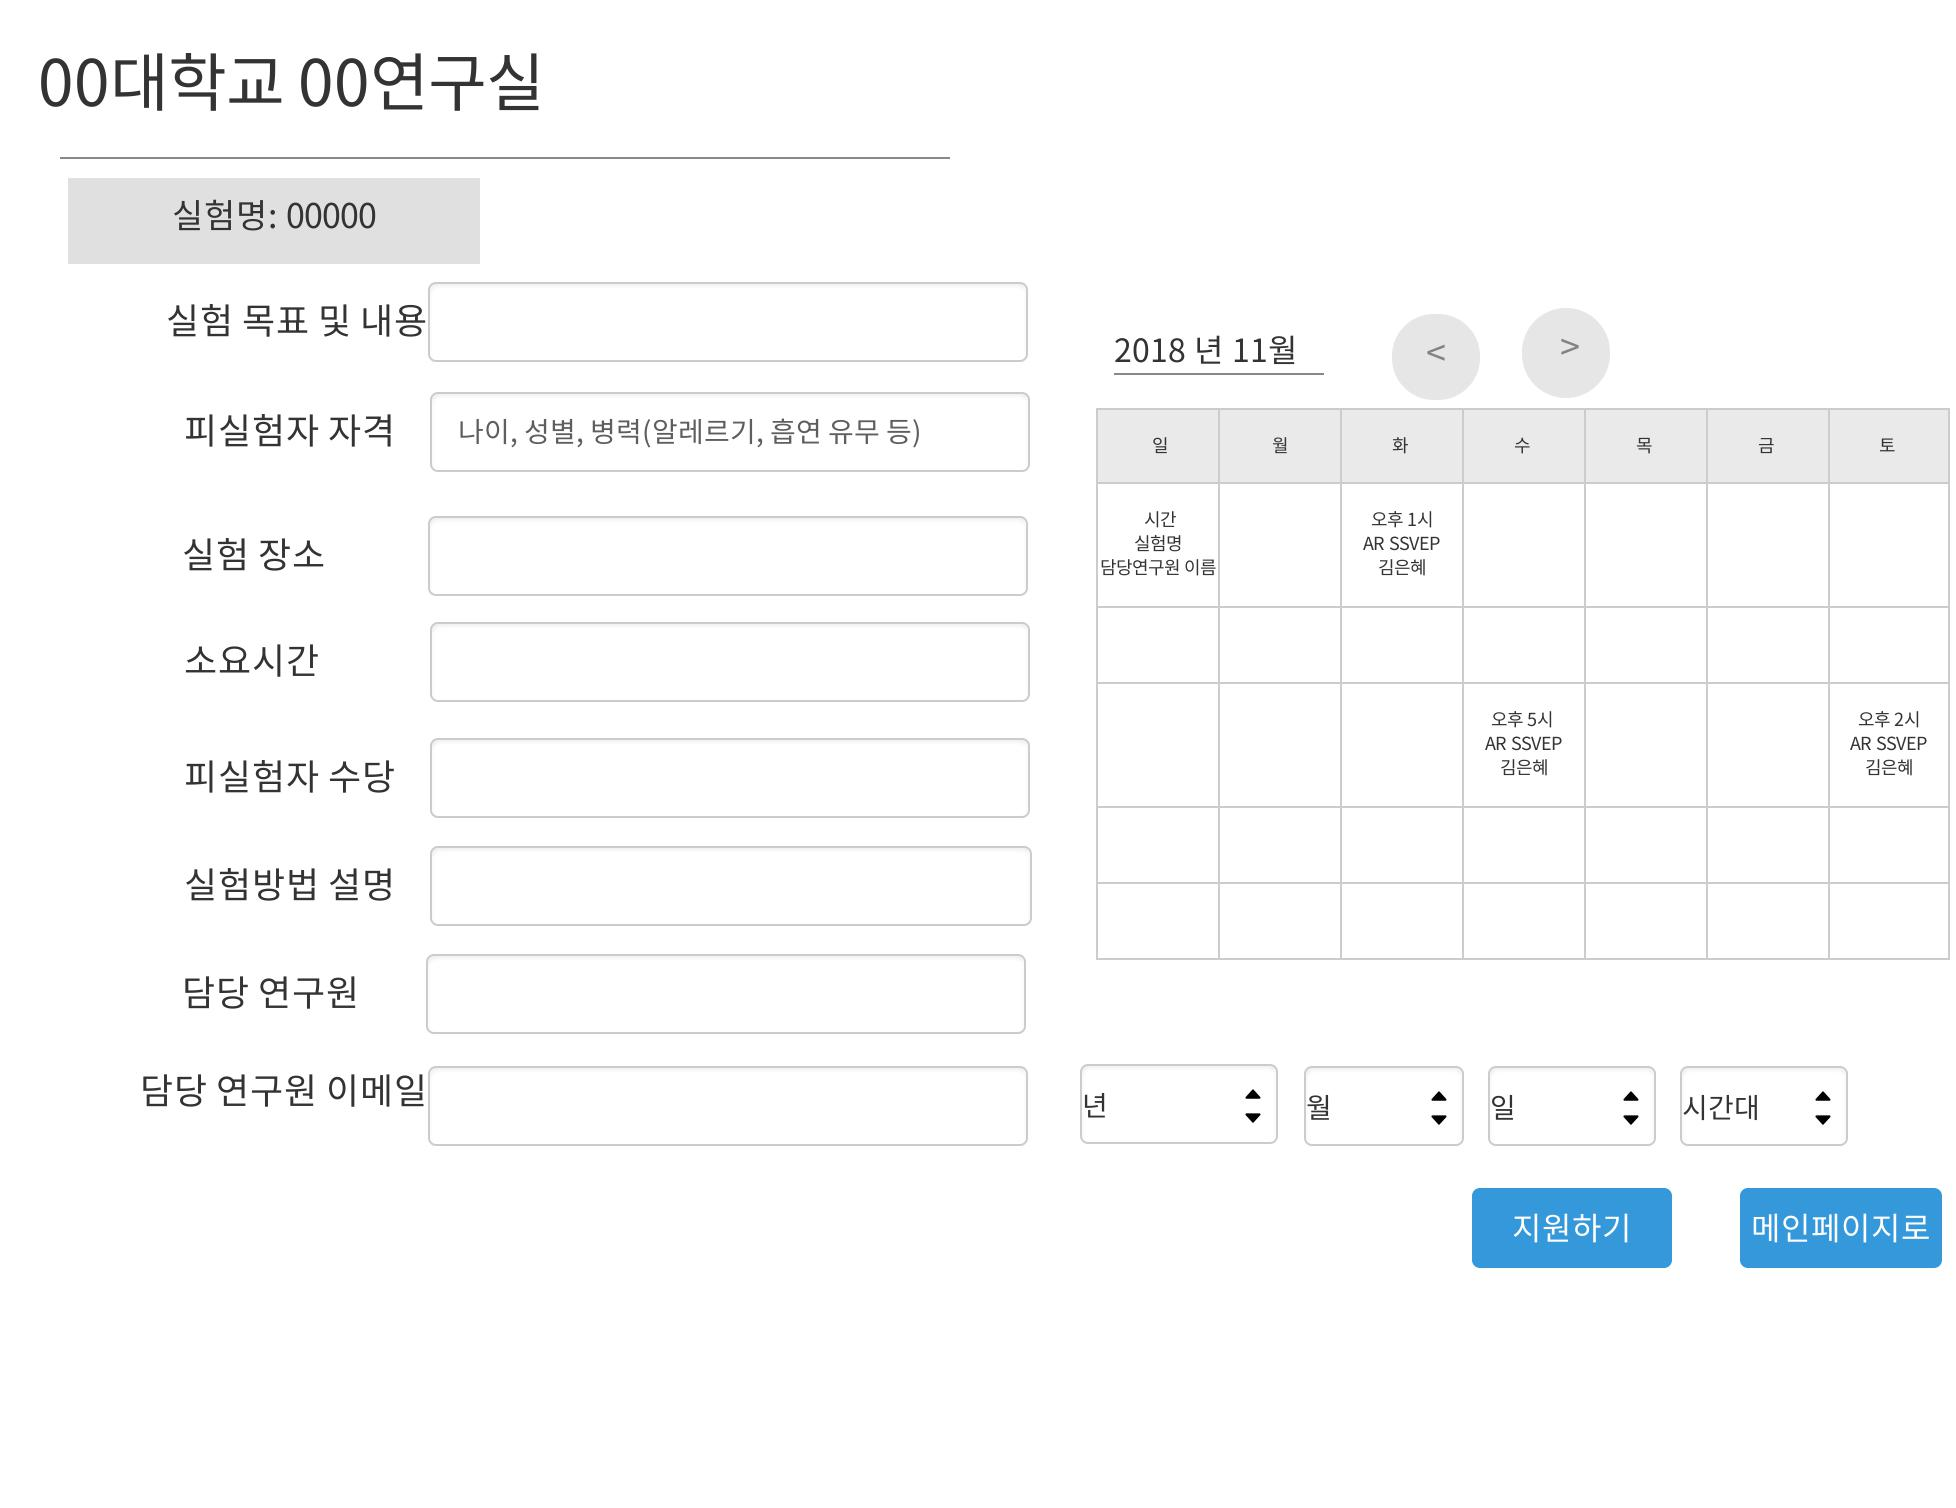
\includegraphics[width=6cm]{Oven/12_detailedExperiment.jpg}
\\Information of the experiment will be shown in the form as below image. Applicants should click a date and time then click the apply button. Their personal information which is entered at sign up phase will be transferred to lab. 

\section{Communication Between Applicants and Lab}
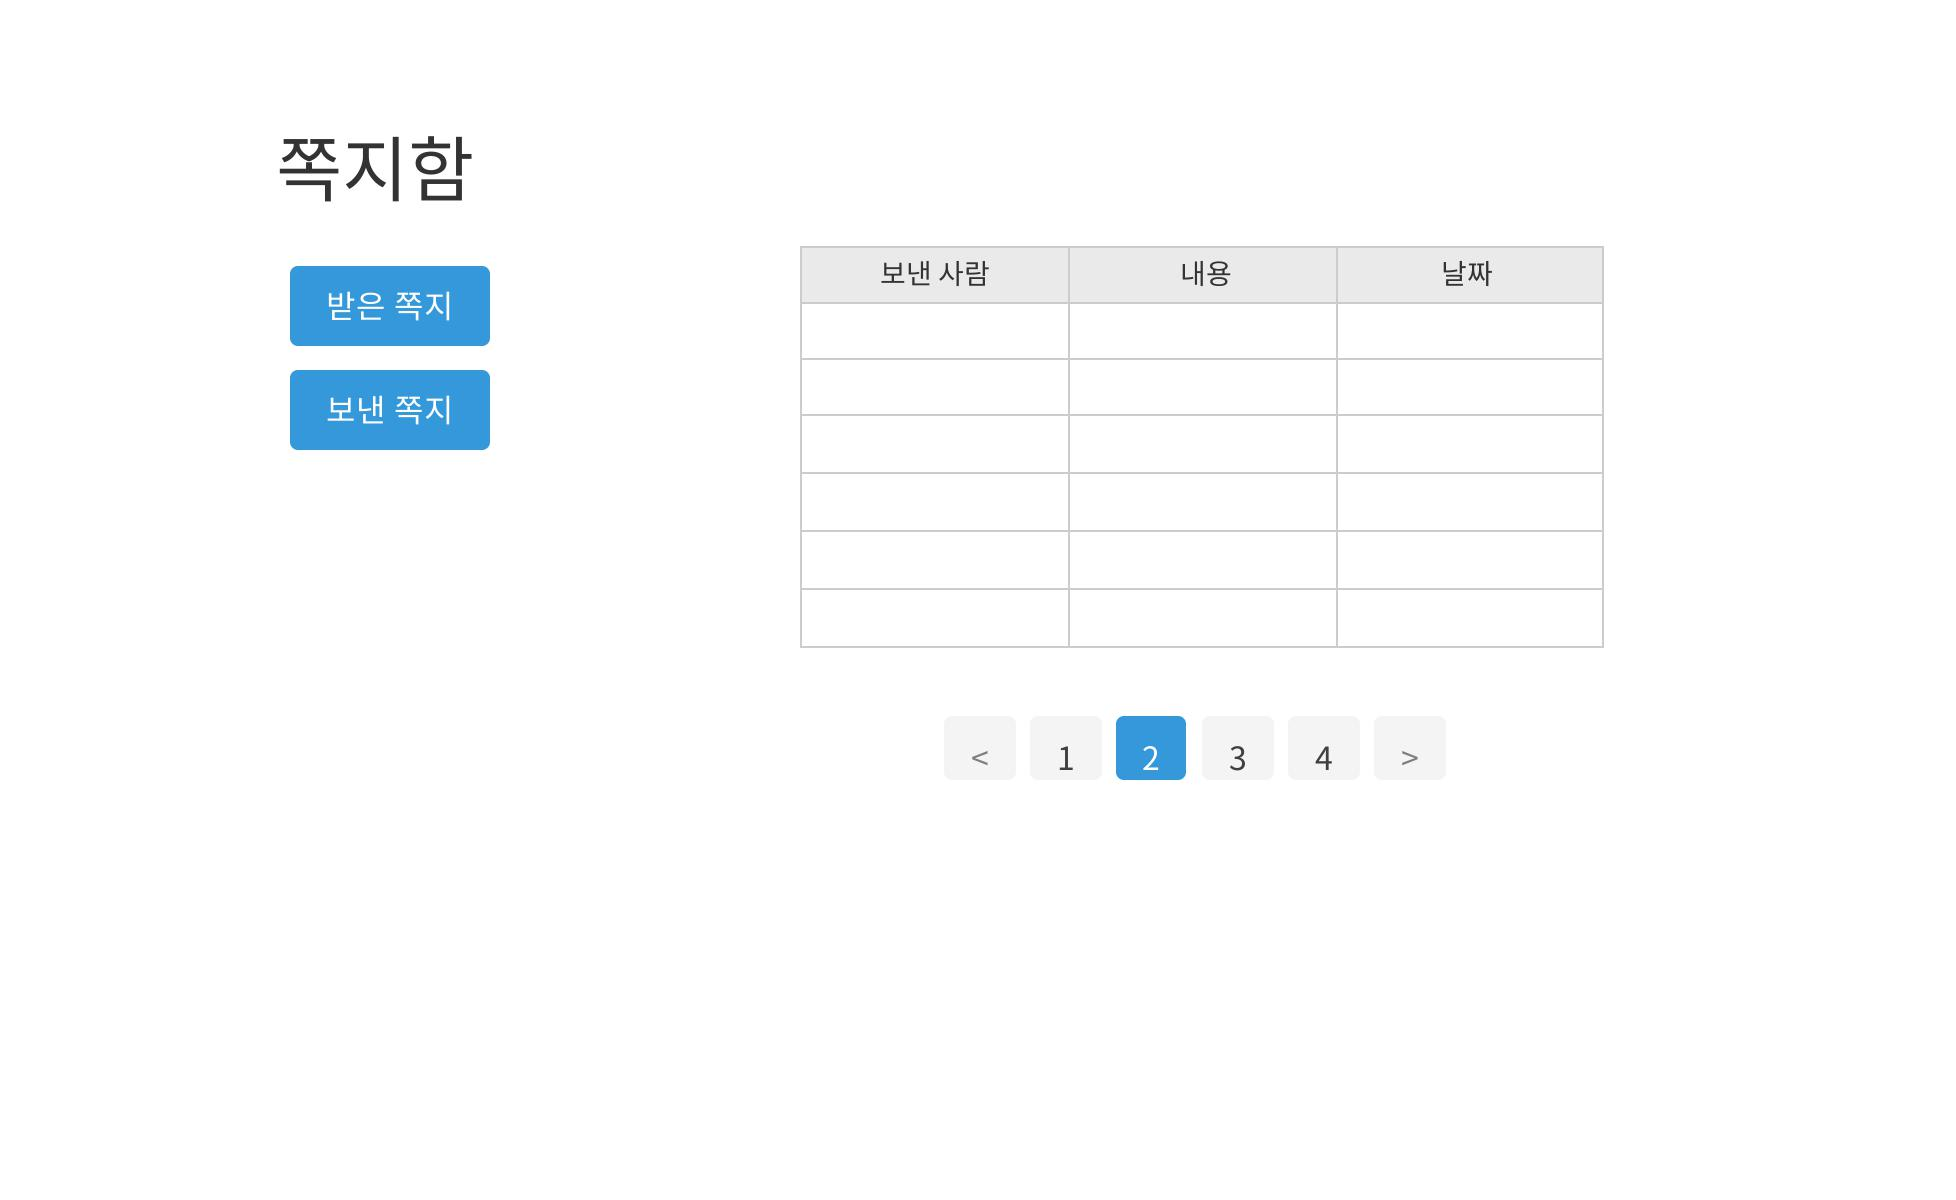
\includegraphics[width=6cm]{Oven/13_dropbox.jpg}
\\All the members regardless of their type will get their own drop box.
\addtolength{\textheight}{-12cm}   % This command serves to balance the column lengths
                                  % on the last page of the document manually. It shortens
                                  % the textheight of the last page by a suitable amount.
                                  % This command does not take effect until the next page
                                  % so it should come on the page before the last. Make
                                  % sure that you do not shorten the textheight too much.

%%%%%%%%%%%%%%%%%%%%%%%%%%%%%%%%%%%%%%%%%%%%%%%%%%%%%%%%%%%%%%%%%%%%%%%%%%%%%%%%



%%%%%%%%%%%%%%%%%%%%%%%%%%%%%%%%%%%%%%%%%%%%%%%%%%%%%%%%%%%%%%%%%%%%%%%%%%%%%%%%



%%%%%%%%%%%%%%%%%%%%%%%%%%%%%%%%%%%%%%%%%%%%%%%%%%%%%%%%%%%%%%%%%%%%%%%%%%%%%%%%




%%%%%%%%%%%%%%%%%%%%%%%%%%%%%%%%%%%%%%%%%%%%%%%%%%%%%%%%%%%%%%%%%%%%%%%%%%%%%%%%










\end{document}
